\documentclass[11pt,psfig,times]{article}
\voffset=-2.2cm
\hoffset=-2.1cm

\setlength{\textwidth}{16.8cm}
\setlength{\textheight}{22.8cm}

\usepackage{latexsym}
\usepackage{epsfig}
\usepackage{times}
\usepackage{enumerate}
\usepackage{bm}
\usepackage{enumitem}
\usepackage{tikz}
\usepackage{amsthm, amsmath,amsfonts, amssymb}
\usepackage{algorithm,algorithmic}
\usepackage{tikz-network}
\usepackage{color}
\usepackage{tabularx}

\usetikzlibrary{hobby}
\definecolor{lightblue}{RGB}{158,202,225}

\renewcommand{\thefootnote}{\fnsymbol{footnote}}
\renewcommand{\baselinestretch}{1.1}

\newcommand{\ignore}[1]{{}}
\newtheorem{theorem}{Theorem}[section]
\newtheorem{corollary}{Corollary}[section]
\newtheorem{lemma}{Lemma}[section]
\newtheorem{observation}{Observation}
\newtheorem{claim}{Claim}
\newtheorem{proposition}{Proposition}
\newtheorem{definition}{Definition}[section]
\newtheorem{fact}{Fact}


\begin{document}
\title{Near-Optimal Network Design with Selfish Agents}
\author{Nuo Xu\thanks {Department of Computer Science, Technical University of Munich. {\tt ge74mis@tum.de}}}
\date{25.11.2024}
\maketitle

\section{Introduction}

\subsection{Classic Generalized Steiner Tree and Steiner Forest problem}
In the classic generalized Steiner tree, we are given an undirected graph \(G = (V,E)\) with non-negative edge cost \(c_e \geq 0\) for every edge $c_e \in E$ and a set of terminals $R \subseteq V $. The goal is to compute the minimum-cost subgraph that spans all terminals. Whereas in the Steiner forest problem, we are given a collection of disjoint subsets of \(V: V_1,V_2,V_3,...V_n\). The goal is to compute a subgraph that any two vertices that belong to the same subset \(V_i\) are connected. 

The Steiner Tree problem is a Steiner Forest problem with a single subset of \(V\). We will denote the optimal solution of both problems as OPT. Finding OPT is NP-hard. 

\subsection{Introduction of Selfish Agents}
In real life, the design of network often involves selfish agents. Imaging the train routes among major cities in Europe, Paris, Munich, Berlin, and Milan. Every city would like to connect to all other cities. However, there won't be a single company that can design the minimum cost network and implement such network. Instead, every city would like to seek the route that they can pay less rather than the route that requires more. 
\begin{figure}
	\begin{center}
	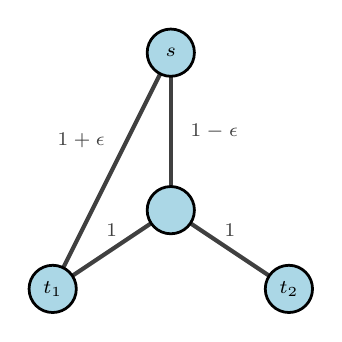
\begin{tikzpicture}
	\Vertex[label=$t_1$]{t1}
	\Vertex[label=$t_2$,x=3]{t2}
	\Vertex[x=1.5,y=1]{middle}
	\Vertex[x=1.5,y=3,label=$s$]{s}
	\Edge[label=$1$,position={above=1mm}](t1)(middle)
	\Edge[label=$1$,position={above=1mm}](t2)(middle)
	\Edge[label=$1-\epsilon$,position={right = 2mm}](s)(middle)
	\Edge[label=$1+\epsilon$,position={above left=2mm}](t1)(s)
	\end{tikzpicture}

\end{center}
\end{figure}

Given an undirected graph \(G\) with non-negative edge costs and \(N\) players, each player is interested in connecting a set of terminals (nodes in \(G\)) via buying a subgraph of \(G\). Players offer each edge in \(G\) certain amount of money, and they would like to pay a little as possible. 

\subsection{Formal Definition of Connection Game}
Here we formally define the connection game for \(N\) players as following:
\begin{itemize}
	\item An undirected graph \(G = (V,E)\).
	\item Non-negative edge cost \(c_e \geq 0\) for every edge $c_e \in E$.
	\item A subset of \(V\) for each player that they must connect to. 
	\item A payment function \(p_i\) indicates that player's payment strategy. \(p_i(e)\) is the contribution that player \(i\) would like to offer for edge \(e\).
\end{itemize}

If the sum of payment on certain edge \(e\) is larger than the cost on that edge \(c_e\), this edge is considered as bought and can be used by all players no matter they contribute to it or not. The goal of all players is to connect all of their terminals. If in the end, a player's terminates are not fully connected, they will face an infinite penalty.  

\section{Nash Equilibrium in Connection Game}
\subsection{Existence of Pure Nash Equilibrium}

A crucial idea of modern game theory introduced by von Neumann is mixed strategies i.e. randomization of pure strategies. Von Neumann's work mostly stayed in zero-sum games. John Nash further extended game theory into \(N\) players general games.  
\begin{theorem}[Nash's theorem]
	With randomization, any game with finite number of players and actions has a mixed-strategy of Nash equilibrium.
\end{theorem}

\begin{definition}[Nash Equilibrium in Connection Game]
	A Nash equilibrium of the connection game is a payment function p such that, if players offer payments \(p\), no payer has an incentive to deviate from their payment. 
\end{definition}

Nash's theorem states that any finite game has at least one mixed strategies Nash equilibrium but no grantee on pure strategy equilibrium. Here it is not hard to see that pure Nash equilibrium may not exist in the connection game. 
 

\subsection{Some Properties of Nash Equilibrium in Connection Game}

\begin{itemize}
	\item \(G_p\) is a forest.
	\item Let \(T^i\) be the smallest tree in \(G_p\) connecting all terminals of player \(i\), then player \(i\) only contributes to edges in \(T^i\).
	\item Each edge is either bought or not at all. 
\end{itemize}

\subsection{Fractional Nash Equilibrium}
\begin{definition}[Fractional Nash Equilibrium]If Nash equilibrium requires players to split cost of some edge, such Nash Equilibrium is fractional.	
\end{definition}


\subsection{Price of Anarchy and Stability}
As mentioned in Section 1, the introduction of selfish agents can lead to worse equilibrium than the best centralized optimum. The question is how bad an equilibrium can be.
\begin{definition}[Price of Anarchy] The price of anarchy of connection game is defined as the ratio of the cost of worst Nash equilibrium over the best centralized design.
	\[P_A = \dfrac{\sum_{1}^{N}p_i(e) }{OPT}\]
\end{definition}

The price of anarchy can be as worst as \(N\).

\begin{definition}[Price of Stability] Price of stability is a complementary concept of price of anarchy which evaluate how good the best equilibrium can be. 

\[P_A = \dfrac{\sum_{1}^{N}p_i(e) }{OPT}\]
\end{definition}

\section{Single Source Games}
\subsection{Definition of Single Source Games}
We have already known that pure Nash Equilibrium might not exist in the general version of connection game i.e. N players with multiple terminals that they would like to connect. We have also already learned that determining the existence of Nash equilibrium in connection game is NP-hard. However, in the single source connection game, Nash equilibrium is determined to exist.

In the single source game, we only allow every player \(i\) has one unique terminal \(t_i\)that they all would like to connect a common terminal \(s\). This can be considered as a special version of Steiner tree problem where \(R = \{s,t_0,t_1,...t_N\}\). 

\begin{definition}[Single source Game]
	A single source game is a game in which all players share a common terminal \(s\) and in addition, each player \(i\) has exactly one other terminal \(t_i\).
\end{definition}

As we have talked before, it is not much of our interests to study the worst equilibrium as it can be really bad. Instead, we would like to see how good the best equilibrium can be. One natural thought is can we achieve an equilibrium that equals to the \(OPT\)? Now suppose the minimum cost Steiner tree \(T^*\) over all players' terminals is given on a sliver plate, we are going to drive an algorithm that gradually assigns each player \(i\) a payment strategy on edge \(e\). Then we are going to prove that the final payment function \(p\) will end up as an equilibrium and yield price of stability as 1.  

It is trivial to see that every leaf node in \(T^*\) is a terminal as if not it is possible to simply discard this node and corresponding edge without affecting the connection of any terminals.
\begin{fact}
	Every leaf node in \(T^*\) is a terminal. 
\end{fact}

\subsection{Payment Strategy Design}
We know that we are going to assign every edge in \(T^*\) but the problem is which edge we are going to assign first. The intuition is to assign edges that are known for sure which players are interested in. First, let \(T^*\) be rooted from \(s\). We will visit \(T^*\) in reverse breadth-first-search order. For every edge \(e\), suppose \(e\) is removed from \(T^*\), \(T^*\) will be divided into two subtrees. Let the subtree that does not contain \(s\) be \(T_e\) and the one contains \(s\) be \(T_s\). It is clear to see that players in \(T_s\) would not be interested in paying anything for \(e\) as discarding \(e\) will not affect their connection to \(s\) at all. Suppose a player can only connect to \(s\) through one path that no edges are shared by any other players, they would have to pay the full cost of every edge on that path. The main loop in our algorithms goes as following: we loop every edge \(e \in T^*\) in reserve BFS order, then for every player \(i \in T_e\) we determine \(p_i(e)\).

\begin{figure}
	\begin{center}
		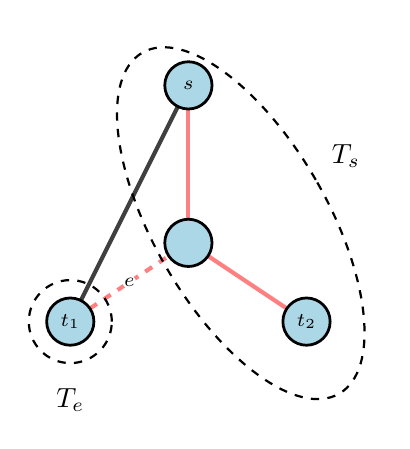
\begin{tikzpicture}
			\Vertex[label=$t_1$]{t1}
			\Vertex[label=$t_2$,x=3]{t2}
			\Vertex[x=1.5,y=1]{middle}
			\Vertex[x=1.5,y=3,label=$s$]{s}
			\Edge[style={dashed},label=$e$,color=red!50,fontcolor=black](t1)(middle)
			\Edge[color=red!50](t2)(middle)
			\Edge[color=red!50](s)(middle)
			\Edge(t1)(s)
			\draw[dashed,thick](0,0) circle (15pt);
			\node at (0, -1) {$T_e$};
			\draw[dashed,thick,rotate=30,label=$T_s$](2.5,0) ellipse(1.1cm and 2.5cm);
 			\node at (3.5, 2.1) {$T_s$};
		\end{tikzpicture}
	\end{center}
\end{figure}

Next we going to assign \(p_i(e)\) so that players would stay in \(T^*\). In every iteration, we modify the cost of every edge according to the following rules:
\begin{itemize}
	\item edges \(f \in T_e\) cost \(p_i(f)\)
	\item edges \(f \in T^*\setminus T_e\) costs 0
	\item edges \(f\notin T^*\) cost \(c(f)\)
\end{itemize}
Then we find the cheapest alternative path \(A_i\) from \(t_i\) to \(s\) from \(F\setminus \{e\}\) under modified cost. 
Now we consider the cost player \(i\) needs to pay if they choose to deviate, \(c(A_i) - \sum_{f\in T^*}p_i(T^*)\), and \(c(e) - \sum_{j\in T_i,j\neq i}p_j(e)\). By choosing the minimum between these two values, we ensure that player \(i\) will never contribute to \(e\) more than the cost of deviation. In another word, it is always  cheaper for players to stay in \(T^*\). Therefore, \(p\) is indeed a Nash equilibrium. 
\begin{corollary}
	The final payment function produced by the above algorithm is indeed a Nash equilibrium.
\end{corollary}

\subsection{Proof of Price of Stability Always Being 1}
We have learned that every player is not going to buy any other edges that are not in \(T^*\). 
To prove that the price of stability is always 1, we need to demonstrate that in the end of the game, every edge in \(T^*\) is fully paid. 
  

To prove that every edge in \(T^*\) is fully paid in the end, we are going to assume that the following lemma is true. 

Suppose \(A_i\) is \(i\)'s alternative path at some stage of the algorithm. Then suppose there are two nodes \(v\) and \(w\) on \(A_i\) that divides this path into three parts. Let edges on \(A_i\) from \(t_i\) to \(v\) be \(f_1\), from \(v\) to \(w\) be \(f_2\), from \(w\) to \(s\) be \(f_3\).
\begin{lemma}
	There must exist a pair of \(\{v,w\}\) such that \(f_1 \in T_e\), \(f_2 \notin T^*\), \(f_3 \in T^*\setminus T_e\).
\end{lemma}
Once \(A_i\) leaves \(T_e\), it will never go back to \(T_e\) again.
\begin{figure}
	\begin{center}
		\begin{tikzpicture}
			\coordinate (s) at (2,2);
			\coordinate (t_1) at (-5,-5);
			\coordinate (t_2) at (-4,-5);
			\coordinate (t_3) at (-3,-5);
			\coordinate (t_4) at (-2,-5);
			\node[draw,circle,fill=lightblue,thick,minimum size=8pt] (CircleNode) at (s)  {s};
			\node[draw,circle,fill=lightblue,thick,minimum size=8pt] (CircleNode) at (t_1)  {s};
			\node[draw,circle,fill=lightblue,thick,minimum size=8pt] (CircleNode) at (t_2)  {s};
			\node[draw,circle,fill=lightblue,thick,minimum size=8pt] (CircleNode) at (t_3)  {s};
		\end{tikzpicture}
	\end{center}
\end{figure}
Suppose \(A_i\) goes from \(T_e\) to \(E\setminus T^*\) then back to \(T_e\), we can find a cheaper alternative path. 
Define \(x\) as the node before \(A_i\) going back to \(T_e\) again. 
Define \(y\) to be the lowest common ancestor of \(x\) and \(t_i\).

\begin{figure}
	\begin{center}
		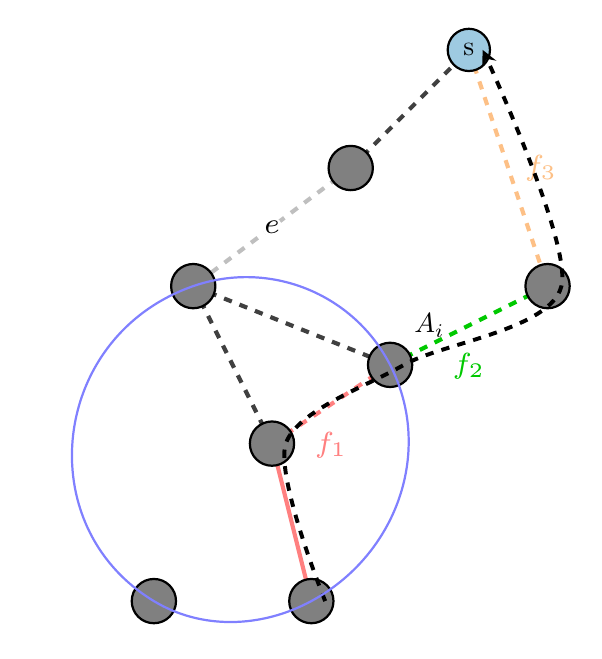
\begin{tikzpicture}
			\coordinate (s) at (2,2);
			\coordinate (e_upper) at (0.5,0.5);
			\coordinate (e_lower) at (-1.5,-1);
			\coordinate (t_i) at (0,-5);
			\coordinate (t_1) at (-2,-5);
			\coordinate (t_iup) at (-0.5,-3);
			\coordinate (u) at (3,-1);
			\coordinate (v) at (1,-2);
			\node[draw,circle,fill=lightblue,thick,minimum size=8pt] (CircleNode) at (s)  {s};
			\draw[thick,black,fill=gray] (t_1) circle (8pt);
			\draw[thick,black,fill=gray]  (e_upper) circle (8pt);
			\draw[thick,black,fill=gray]  (e_lower) circle (8pt);
			\draw[thick,black,fill=gray]  (t_i) circle (8pt);
			\draw[thick,black,fill=gray]  (t_iup) circle (8pt);
			\draw[thick,black,fill=gray]  (u) circle (8pt);
			\draw[thick,black,fill=gray]  (v) circle (8pt);
			\Edge[style={dashed},label=$e$,fontcolor=black,fontscale =1.5,color=gray!50](e_upper)(e_lower)
			\Edge[style={dashed}](e_lower)(t_iup)
			\Edge[style={dashed}](e_lower)(v)
			\Edge[style={dashed}](e_upper)(s)
			\Edge[color=red!50](t_i)(t_iup)
			\Edge[style={dashed},color=red!50,label=$f_1$,position={below=2mm},fontscale=1.5](t_iup)(v)
			\Edge[style={dashed},RGB,color={0,201,0},label=$f_2$,position={below=2mm},fontscale=1.5](v)(u)
			\Edge[style={dashed},RGB,color={253,192,134},label=$f_3$,position={above=2mm,right=1mm},fontscale=1.5](s)(u)
			\draw[line width=0.5mm,dashed,-stealth] plot[smooth] coordinates {([xshift=5pt]t_i)([xshift=5pt]t_iup)([xshift=5pt]v) ([xshift=5pt]u) ([xshift=5pt]s)};
			\node at (1.5,-1.5){$A_i$};
			\draw[color=blue!50,thick] (e_lower) to[closed, curve through = {(v)(t_i)(t_1)}] (e_lower); 
			
		\end{tikzpicture}
	\end{center}
\end{figure}

\begin{lemma}
	All edges in \(T^*\) are bought, i.e. $\sum p_i(e) = c(e)$ for any $e \in T^*$.
\end{lemma}

Suppose there exists some edge \(e\) such that after all players in \(T_e\) have contributed to that edge, \(p_i(e) < c(e)\), we can prove that \(T_e\) costs more than \(\bigcup_{i\in T_e} A_i\) which is a contradiction of \(T^*\) is \(OPT\).



\subsection{Approximate Nash Equilibrium}
Although we proved that the determined existence of Nash equilibrium in single source game, the algorithm presented is not feasible as the finding the minimum cost Steiner tree is NP-hard by itself. 
\begin{definition}[Approximate Equilibrium]
	A \((1+\epsilon)\)-approximate Nash Equilibrium is a payment function \(p\) such that player \(i\) would not deviate their payment by a factor of \(1+\epsilon\).
\end{definition}

\begin{theorem}
	Given a single source game and \(\alpha\) approximation of minimum-cost Steiner tree \(T\), 
\end{theorem}

\subsection{How to Assign \(p_i(e)\)?}
In every iteration, we modify the cost of every edge according to the following rules:
	\begin{itemize}
		\item let costs of edges \(e \in T_e\) be \(p_i(e)\)
		\item let costs of edges \(e \in T_s\) be  0
		\item costs of edges \(e\notin T^*\) stay the same
	\end{itemize}
	
	We can find the cheapest alternative path \(A_i\) from \(t_i\) to \(s\) from \(G \setminus \{e\}\) under modified cost in polynomial time. 
		Find the minimum value of:
		\begin{itemize}
			\item $c(e) - $ contribution from other players to edge \(e\)
			\item cost of \(A_i-\) sum of all contribution of player \(i\) to \(T^*\) 
		\end{itemize}
	
	
	\subsection{Algorithm for Assigning $p_i(e)$}
	\begin{algorithm}[H]
	\begin{algorithmic}[1]
		\STATE $p_i(e) \gets 0, \forall t_i \in R, \forall e \in E$ 
		\WHILE{$e \in ReverseBFS(T^*)$}
		\IF{$e$ is a cut} 
		\STATE $p_i(e) \gets c(e)$
		\ELSE
		\STATE \(c(e) \gets p_i(f)  \qquad \forall e \in T_e\) 
		\STATE \(c(e) \gets 0 \qquad \forall e \in T_S\) 
		\STATE $A_i \gets$ the cheapest alternative path from \(s\) to \(t_i\) in $G\setminus\{e\}$ 
		\STATE \(p_i(e) \gets min\{c(A_i) - \sum_{e\in T^*}p_i(e), c(e)-\sum_{j}p_j(e) \}\)
		\ENDIF
		\ENDWHILE
	\end{algorithmic}
	\caption{pseudocode for assigning $p_i(e)$ }
	\label{alg:seq}
	\end{algorithm}
	
	
	
	 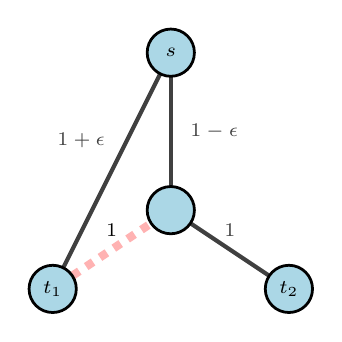
\begin{tikzpicture}
		\Vertex[label=$t_1$]{t1}
		\Vertex[label=$t_2$,x=3]{t2}
		\Vertex[x=1.5,y=1]{middle}
		\Vertex[x=1.5,y=3,label=$s$]{s}
		\Edge[label=$1$,style={dashed},fontcolor=black, color=red!30,position={above=1mm},lw=3pt](t1)(middle)
		\Edge[label=$1$,position={above=1mm}](t2)(middle)
		\Edge[label=$1-\epsilon$,position={right = 2mm}](s)(middle)
		\Edge[label=$1+\epsilon$,position={above left=2mm}](t1)(s)
	\end{tikzpicture}
	 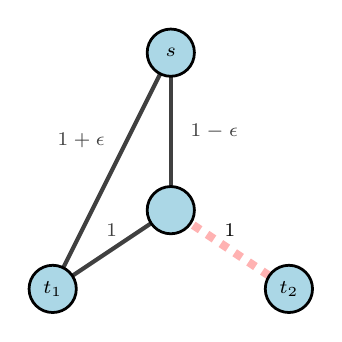
\begin{tikzpicture}
		\Vertex[label=$t_1$]{t1}
		\Vertex[label=$t_2$,x=3]{t2}
		\Vertex[x=1.5,y=1]{middle}
		\Vertex[x=1.5,y=3,label=$s$]{s}
		\Edge[label=$1$,position={above=1mm}](t1)(middle)
		\Edge[label=$1$,,style={dashed},fontcolor=black,lw=3pt,color=red!30,position={above=1mm}](t2)(middle)
		\Edge[label=$1-\epsilon$,position={right = 2mm}](s)(middle)
		\Edge[label=$1+\epsilon$,position={above left=2mm}](t1)(s)
	\end{tikzpicture}
	 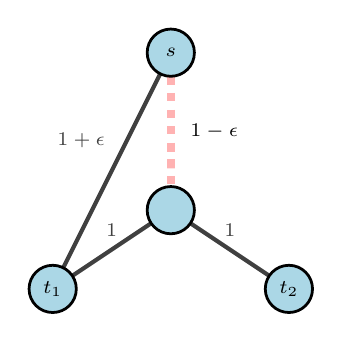
\begin{tikzpicture}
		\Vertex[label=$t_1$]{t1}
		\Vertex[label=$t_2$,x=3]{t2}
		\Vertex[x=1.5,y=1]{middle}
		\Vertex[x=1.5,y=3,label=$s$]{s}
		\Edge[label=$1$,position={above=1mm}](t1)(middle)
		\Edge[label=$1$,position={above=1mm}](t2)(middle)
		\Edge[label=$1-\epsilon$,,style={dashed},fontcolor=black,lw=3pt,color=red!30,position={right = 2mm}](s)(middle)
		\Edge[label=$1+\epsilon$,position={above left=2mm}](t1)(s)
	\end{tikzpicture}\\
	$e$ is not a cut.\\
	consider $c(A_1) = 1+\epsilon, \quad p_1(T^*) = 0$\\
	$c(e) = 1, \quad  \sum_{j}p_j(e) = 0$\\
	set $p_1(e) = 1$
	$e$ is a cut.\\
	set $p_2(e) = 1$
	$e$ is not a cut.\\
	\textbf{for $t_1$}\\
	$c(A_1) = 1+\epsilon, \quad  p_1(T^*) = 1$\\
	$c(e) = 1-\epsilon, \quad \sum_{j}p_j(e) = 0$\\
	set $p_1(e) = \epsilon$\\
	\textbf{for $t_2$}\\
	$c(A_2) = 3+\epsilon, \quad p_2(T^*) = 1$\\
	$c(e) = 1-\epsilon,\quad  \sum_{j}p_j(e) = \epsilon$\\
	set $p_2(e) = 1-2\epsilon$
	
	
\subsection{Proof of \(p\) Being Nash Equilibrium}
	\begin{corollary}
		If $T^*$ is fully paid in the end of the game, the final payment function produced by the above algorithm is indeed a Nash equilibrium.
	\end{corollary}
	By assigning $p_i(e) = min\{c(A_i) - \sum_{e\in T^*}p_i(T^*), c(e) - \sum_{j\in T_i,j\neq i}p_j(e)\}$, we ensure that player \(i\) will never contribute to \(e\) more than the cost of deviation. \\
	In another word, it is never player $i$'s interests to deviate from buying $e$. And this holds true for every player in every edge in $T^*$. Therefore, \(p\) is indeed a Nash equilibrium. 
	
	First, assume that the following lemma is true. 
	Suppose \(A_i\) is \(i\)'s alternative path at some stage of the algorithm. Then suppose there are two nodes \(v\) and \(w\) on \(A_i\) that divides this path into three parts. Let edges on \(A_i\) from \(t_i\) to \(v\) be \(f_1\), from \(v\) to \(w\) be \(f_2\), from \(w\) to \(s\) be \(f_3\).
	\begin{lemma}
		There must exist a pair of \(\{v,w\}\) such that \(f_1 \in T_e\), \(f_2 \notin T^*\), \(f_3 \in T_s\).
	\end{lemma}
	
	
	\textbf{Prove $T^*$ is fully paid via contradiction.}
	
	
	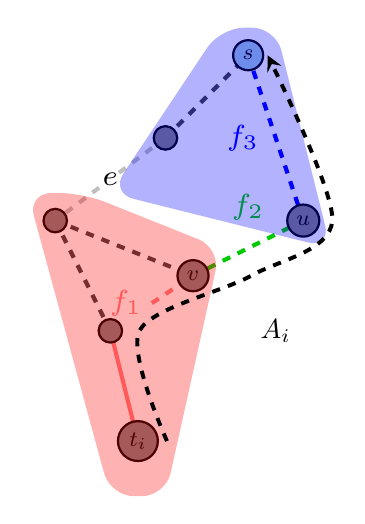
\begin{tikzpicture}[scale=0.7]
		\coordinate (s) at (2,2);
		\coordinate (e_upper) at (0.5,0.5);
		\coordinate (e_lower) at (-1.5,-1);
		\coordinate (t_i) at (0,-5);
		\coordinate (t_1) at (-2,-5);
		\coordinate (t_iup) at (-0.5,-3);
		\coordinate (u) at (3,-1);
		\coordinate (v) at (1,-2);
		\node[draw,circle,fill=lightblue,thick,inner sep=2pt,minimum size=5pt] (CircleNode) at (s)  {\footnotesize $s$};
		\node[draw,circle,fill=gray,thick,inner sep=2pt,minimum size=5pt] (CircleNode) at (t_i)  {\footnotesize $t_i$};
		\node[draw,circle,fill=gray,thick,inner sep=3pt,minimum size=5pt] (CircleNode) at (e_upper){};
		\node[draw,circle,fill=gray,thick,inner sep=3pt,minimum size=5pt] (CircleNode) at (e_lower){};
		\node[draw,circle,fill=gray,thick,inner sep=3pt,minimum size=5pt] (CircleNode) at (t_iup){};
		\node[draw,circle,fill=gray,thick,inner sep=2pt,minimum size=5pt] (CircleNode) at (u){\footnotesize $u$};
		\node[draw,circle,fill=gray,thick,inner sep=2pt,minimum size=5pt] (CircleNode) at (v){\footnotesize $v$};
	
		\draw [ draw=none,rounded corners = 3mm,fill=red,fill opacity=0.3]([shift={(-0.5,0.5)}]e_lower)--([shift={(0.5,0.5)}]e_lower)--([shift={(0.5,0.5)}]v)--([shift={(0.5,-1)}]t_i)--([shift={(-0.5,-1)}]t_i)--cycle;
	
		\draw [ draw=none,rounded corners = 3mm,fill=blue,fill opacity=0.3]([shift={(0.5,0.5)}]s)--([shift={(0.5,-0.5)}]u)--([shift={(-1,-1)}]e_upper)--([shift={(-0.5,0.5)}]s)--cycle;  
	
		\Edge[style={dashed},label=$e$,fontcolor=black,fontscale =1.5,color=gray!50](e_upper)(e_lower)
		\Edge[style={dashed}](e_lower)(t_iup)
		\Edge[style={dashed}](e_lower)(v)
		\Edge[style={dashed}](e_upper)(s)
		\Edge[color=red!50](t_i)(t_iup)
		\Edge[style={dashed},color=red!50,label=$f_1$,position={above=1.5mm,left=0.1mm},fontscale=1.5](t_iup)(v)
		\Edge[style={dashed},RGB,color={0,201,0},label=$f_2$,position={above=2mm},fontscale=1.5](v)(u)
		\Edge[style={dashed},color=blue,label=$f_3$,position={above=2mm,left=1mm},fontscale=1.5](s)(u)
		\draw[line width=0.5mm,dashed,-stealth] plot[smooth] coordinates {([xshift=15pt]t_i)([xshift=15pt]t_iup)([xshift=30pt]v) ([xshift=15pt]u) ([xshift=10pt]s)};
		\node at (2.5,-3){$A_i$};
		% \draw[color=blue!50,thick] (e_lower) to[closed, curve through = {(v)(t_i)(t_1)}] (e_lower); 
	\end{tikzpicture}
	  

\subsection{Proof $T^*$ is fully paid}
	\begin{lemma}
		All edges in \(T^*\) are bought, i.e. $\sum p_i(e) = c(e)$ for any $e \in T^*$.
	\end{lemma}
	Suppose there exists some edge \(e\) such that after all players in \(T_e\) have contributed to that edge, \(p_i(e) < c(e)\), we can prove that \(T_e\) costs more than \(\bigcup_{i\in T_e} A_i\) which is a contradiction of \(T^*\) is \(OPT\).
	
		\begin{definition}
			For each player $i$, name the highest ancestor of $t_i$ in $A_i$ that is also in $T_e$, player $i$'s deviation point, denoted $d_i$. Let $T_i$ be the subtree rooted from $d_i$.
		\end{definition}
		
		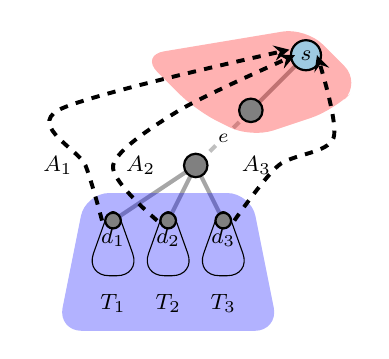
\begin{tikzpicture}[scale=0.7]
			\coordinate (s) at (1.5,2);
			\coordinate (d1) at (-2,-1);
			\coordinate (d2) at (-1,-1);
			\coordinate (d3) at (0,-1);
			\coordinate (e_upper) at (0.5,1);
			\coordinate (e_lower) at (-0.5,0);
			
			\draw [ draw=none,rounded corners = 3mm,fill=blue,fill opacity=0.3] ([shift={(-1,-2)}]d1)--([shift={(1,-2)}]d3)--([shift={(0.5,0.5)}]d3)--([shift={(-0.5,0.5)}]d1)--cycle;  
	
			\draw [ draw=none,rounded corners = 3mm,fill=red,fill opacity=0.3] ([shift={(0,0.5)}]s) --([shift={(1,-0.5)}]s)--([shift={(0.5,-1)}]s)--([shift={(0,-0.5)}]e_upper)--([shift={(-2,-1)}]s)--([shift={(-3,0)}]s)--cycle; 
	
			\node[draw,circle,fill=lightblue,thick,inner sep=2pt,minimum size=5pt] (CircleNode) at (s)  {\footnotesize $s$};
			\node[draw,circle,fill=gray,thick,inner sep=3pt,minimum size=5pt] (CircleNode) at (e_upper){};
			\node[draw,circle,fill=gray,thick,inner sep=3pt,minimum size=5pt] (CircleNode) at (e_lower){};
			\node[draw,circle,fill=gray,thick,inner sep=2pt,minimum size=5pt] (CircleNode) at (d1){};
			\node[draw,circle,fill=gray,thick,inner sep=2pt,minimum size=5pt] (CircleNode) at (d2){};
			\node[draw,circle,fill=gray,thick,inner sep=2pt,minimum size=5pt] (CircleNode) at (d3){};
	
			\Edge[style={dashed},label=$e$,fontcolor=black,color=gray!50](e_upper)(e_lower)
			\Edge[color=gray!70](s)(e_upper)
			\Edge[color=gray!70](d1)(e_lower)
			\Edge[color=gray!70](d2)(e_lower)
			\Edge[color=gray!70](d3)(e_lower)
	
			\draw [rounded corners = 3mm] ([shift={(0,0.4)}]d1)--([shift={(-0.5,-1)}]d1)--([shift={(0.5,-1)}]d1)--cycle;   
			\draw [rounded corners = 3mm] ([shift={(0,0.4)}]d2)--([shift={(-0.5,-1)}]d2)--([shift={(0.5,-1)}]d2)--cycle;
			\draw [rounded corners = 3mm] ([shift={(0,0.4)}]d3)--([shift={(-0.5,-1)}]d3)--([shift={(0.5,-1)}]d3)--cycle;
			
			\node at ([shift={(0,-0.3)}]d1){\footnotesize $d_1$};
			\node at ([shift={(0,-0.3)}]d2){\footnotesize $d_2$};
			\node at ([shift={(0,-0.3)}]d3){\footnotesize $d_3$};
			
			\node at ([shift={(-1,1)}]d1){\footnotesize $A_1$};
			\node at ([shift={(-0.5,1)}]d2){\footnotesize $A_2$};
			\node at ([shift={(0.6,1)}]d3){\footnotesize $A_3$};
	
			\node at ([shift={(0,-1.5)}]d1){\footnotesize $T_1$};
			\node at ([shift={(0,-1.5)}]d2){\footnotesize $T_2$};
			\node at ([shift={(0,-1.5)}]d3){\footnotesize $T_3$};
	
			\draw[line width=0.5mm,dashed,-stealth] plot[smooth] coordinates {([shift={(-0.2,0)}]d1)([shift={(-0.5,1)}]d1)([shift={(-1,2)}]d1)([shift={(-0.3,0.1)}]s)};
			\draw[line width=0.5mm,dashed,-stealth] plot[smooth] coordinates {([shift={(-0.2,0)}]d2)([shift={(-1,1)}]d2)([shift={(0.2,2)}]d2)([shift={(-0.2,0)}]s)};
			\draw[line width=0.5mm,dashed,-stealth] plot[smooth] coordinates {([shift={(0.2,0)}]d3)([shift={(1,1)}]d3)([shift={(2,1.5)}]d3)([shift={(0.2,0)}]s)};  
		\end{tikzpicture}
	   
	
	
	{$d_i$s Are Siblings in \(\bigcup_{i\in T_e} A_i\) }
		\begin{tikzpicture}
			\coordinate (di) at (-2,-2);
			\coordinate (dj) at (-1,-1);
			\coordinate (e_upper) at (0.5,1);
			\coordinate (e_lower) at (-0.5,0);
			\coordinate (tj) at (-1,-4);
			\coordinate (ti) at (-3,-4);
	
			\node[draw,circle,fill=gray!50,thick,inner sep=3pt,minimum size=5pt] (CircleNode) at (e_upper){};
			\node[draw,circle,fill=gray!50,thick,inner sep=3pt,minimum size=5pt] (CircleNode) at (e_lower){};
			\node[draw,circle,fill=gray!50,thick,inner sep=1pt,minimum size=3pt] (CircleNode) at (di){\scriptsize $d_i$};
			\node[draw,circle,fill=gray!50,thick,inner sep=1pt,minimum size=3pt] (CircleNode) at (dj){\scriptsize  $d_j$};
			\node[draw,circle,fill=gray!50,thick,inner sep=1pt,minimum size=3pt] (CircleNode) at (ti){\scriptsize $t_i$};
			\node[draw,circle,fill=gray!50,thick,inner sep=1pt,minimum size=3pt] (CircleNode) at (tj){\scriptsize  $t_j$};
	
			\Edge[style={dashed},label=$e$,fontcolor=black,color=gray!50](e_upper)(e_lower)
			\Edge[color=gray!70](s)(e_upper)
			\Edge[color=gray!70](dj)(e_lower)
			\Edge[color=gray!70](di)(dj)
			\Edge[color=gray!70](di)(tj)
			\Edge[color=gray!70](di)(ti)
	
			\draw[line width=0.5mm,dashed,-stealth] plot[smooth] coordinates {([shift={(-0.2,0)}]ti)([shift={(-0.2,0)}]di)([shift={(-2,3)}]di)};
			\draw[line width=0.5mm,dashed,-stealth] plot[smooth] coordinates {([shift={(0.2,0)}]tj)([shift={(0.2,0)}]di)([shift={(0.2,0)}]dj)([shift={(3,1)}]dj)};           
		\end{tikzpicture}
	
	
	
	\begin{itemize}
		\item    Recall in each step when we decide a payment $p_i(e)$ for player $i$ on $e$, we choose \(p_i(e) \gets min\{c(A_i) - \sum_{e\in T^*}p_i(e), c(e)-\sum_{j}p_j(e) \}\)
		\item If we decide player $i$ needs to pay $c(e)-\sum_{j}p_j(e) $, then $e$ is bought. 
		\item If $e$ is not bought, then we set all players in $T_e$, their payment function on $e$ to be $c(A_i) - \sum_{e\in T^*}p_i(e)$
	\end{itemize}   
	
		\begin{itemize}
		\item Modify $T^*$ by replacing $T_e$ with \(\bigcup_{i\in T_e} A_i\).
		\item All other players leave their payments unchanged.
		\item $A_i$ will be fully paid. 
		\item By the lemma, we know that all players in $T_e$ can stay connect to $s$ after the modification without increasing their expenditures.
		\end{itemize}
	
		\textbf{This is a contradiction to $T^*$ being unique.}

	
	\subsection{Proof of Lemma}
		\begin{lemma}
			\(f_1 \in T_e\), \(f_2 \notin T^*\), \(f_3 \in T_s\).
		\end{lemma}
		Suppose once $A_i$ reaches a node in $T_s$, then all subsequent edges will be in $T_s$ as edges in $T_s$ cost 0 under modified cost. \\
		$A_i$ will always reach a node in $T_s$ since $s \in T_s$.\\
		So we only need to prove that only $A_i$ leaves $T_e$ it will only be in $G\setminus T_e$, i.e. \textbf{$A_i$ does not go back to $T_e$ anymore.} We show this by contradiction. 
		Suppose there are two nodes \(v\) and \(w\) on \(A_i\) that divides the part of $A_i$ before reaching to $T_s$ into three parts such that \(P_1 \in T_e\), \(P_2 \notin T^*\), \(P_4 \in T_e\).\\
	
		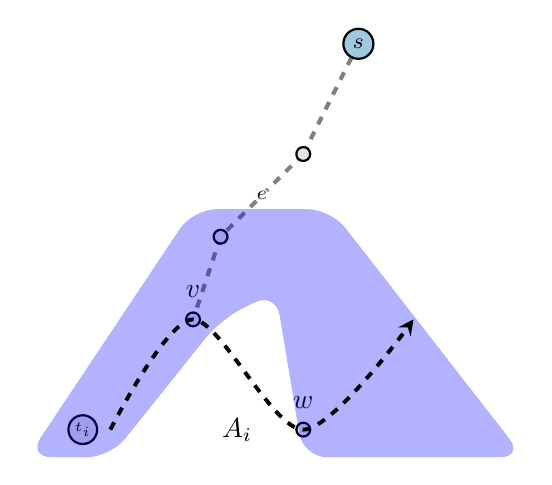
\begin{tikzpicture}[scale=0.7]
			\coordinate (s) at (2,3);
			\coordinate (e_upper) at (1,1);
			\coordinate (e_lower) at (-0.5,-0.5);
			\coordinate (t1) at (-3,-4);
			\coordinate (v) at (-1,-2);
			\coordinate (w) at (1,-4);
	
			\node[draw,circle,fill=lightblue,thick,inner sep=2pt,minimum size=5pt] (CircleNode) at (s)  {\footnotesize $s$};
			\node[draw,circle,fill=gray!20,thick,inner sep=1pt,minimum size=5pt] (CircleNode) at (t1)  {\tiny $t_i$};
			\node[draw,circle,fill=gray!20,thick,inner sep=1pt,minimum size=5pt] (CircleNode) at (v)  {};
			\node[draw,circle,fill=gray!20,thick,inner sep=1pt,minimum size=5pt] (CircleNode) at (w)  {};
			\node[draw,circle,fill=gray!20,thick,inner sep=1pt,minimum size=5pt] (CircleNode) at (e_upper)  {};
			\node[draw,circle,fill=gray!20,thick,inner sep=1pt,minimum size=5pt] (CircleNode) at (e_lower)  {};
			
			\node at ([shift={(0,0.5)}]w){$w$};
			\node at ([shift={(0,0.5)}]v){$v$};
			\node at ([shift={(-1.2,0)}]w){$A_i$};
			\Edge[style={dashed},label=$e$,fontcolor=black,color = gray](e_upper)(e_lower)
			\Edge [style={dashed},color = gray](e_lower)(v)
			\Edge[style={dashed},color = gray](e_upper)(s)
			\draw [draw=none,rounded corners = 3mm,fill=blue,fill opacity=0.3] ([shift={(-0.5,0.5)}]e_lower)--([shift={(-1,-0.5)}]t1)--([shift={(0.5,-0.5)}]t1)--([shift={(0.5,0)}]v)--([shift={(-0.5,2.5)}]w)--([shift={(0,-0.5)}]w)--([shift={(5,-0.5)}]t1)--([shift={(8,-0.5)}]t1)--([shift={(2,0.5)}]e_lower)--cycle; 
	
			\draw[line width=0.5mm,dashed,-stealth] plot[smooth] coordinates {([shift={(0.5,0)}]t1)([shift={(0,0)}]v)([shift={(0,0)}]w)([shift={(2,2)}]w)}; 
		\end{tikzpicture}
		  
	
	
		Let $y$ be the lowest common ancestor of $t_i \text{ and } w \text{ in } T_e$.\\
		We will show that by replacing $P_1 \bigcup P_2$ with $P_3 \bigcup P_4$,
		player $i$ would obtain a better deviation than $A_i$.\\
		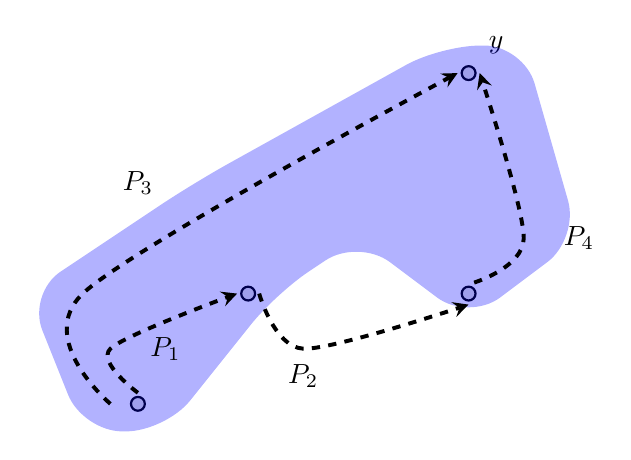
\begin{tikzpicture}[scale=0.7]
			\coordinate (y) at (2,2);
			\node at ([shift={(0.5,0.5)}]y) {$y$};
			\coordinate (v) at (-2,-2);
			\coordinate (w) at (2,-2);
			\coordinate (ti) at (-4,-4);
			\node[draw,circle,fill=gray!20,thick,inner sep=1pt,minimum size=5pt] (CircleNode) at (v)  {};
			\node[draw,circle,fill=gray!20,thick,inner sep=1pt,minimum size=5pt] (CircleNode) at (w)  {};
			\node[draw,circle,fill=gray!20,thick,inner sep=1pt,minimum size=5pt] (CircleNode) at (y)  {};
			\node[draw,circle,fill=gray!20,thick,inner sep=1pt,minimum size=5pt] (CircleNode) at (ti)  {};
	
			\draw [draw=none,rounded corners = 5mm,fill=blue,fill opacity=0.3] ([shift={(-0.5,0.5)}]y)--([shift={(-5,-2)}]y)--([shift={(-2,2)}]ti)--([shift={(-1,-0.5)}]ti)--([shift={(0.5,-0.5)}]ti)--([shift={(0.5,0)}]v)--([shift={(2,1)}]v)--([shift={(0,-0.5)}]w)--([shift={(2,1)}]w)--([shift={(1,0.5)}]y)--cycle; 
	
			\draw[line width=0.5mm,dashed,-stealth] plot[smooth] coordinates {([shift={(-0.5,0)}]ti)([shift={(-1,2)}]ti)([shift={(-0.2,0)}]y)};
			\node at ([shift={(0,4)}]ti) {$P_3$};
			\draw[line width=0.5mm,dashed,-stealth] plot[smooth] coordinates {([shift={(0,0.2)}]ti)([shift={(-0.5,1)}]ti)([shift={(-0.2,0)}]v)};
			\node at (-3.5,-3) {$P_1$};
			\draw[line width=0.5mm,dashed,-stealth] plot[smooth] coordinates {([shift={(0.2,0)}]v)([shift={(1,-1)}]v)([shift={(0,-0.2)}]w)};
			\node at ([shift={(1,-1.5)}]v){$P_2$};
			\draw[line width=0.5mm,dashed,-stealth] plot[smooth] coordinates {([shift={(0.1,0.2)}]w)([shift={(1,1)}]w)([shift={(0.2,0)}]y)};
			\node at ([shift={(2,1)}]w){$P_4$};
		\end{tikzpicture}
	
	
	
		\begin{claim}
			$ c^{'}(P_4) = p_i(P_4) = 0$ for $i$.
		\end{claim}
		\begin{itemize}
			\item None of edges in $P_4$ are on player $i$'s path from $t_i$ to $s$.
		\end{itemize}
		\begin{claim}
		$P_1$ is restrictly below $y$,i.e. $P_1$ is a subpath of $P_3$. 
		\end{claim}
		\begin{itemize}
			\item If not, $P_3$ is just a subpath of $P_1$. 
			\item $c^{'}(P_3) \leq c^{'}(P_1) \text{ and } c^{'}(P_4) = 0$.
			\item $ c^{'}(P_3\bigcup P_4) \leq c^{'}(P_1\bigcup P_2).$ 
		\end{itemize}
	
	
		\begin{itemize}
			\item When deciding the payment of each edge in $P_3$, $p_i(e) \leq c(A_i)$
			\item At any time, player $i$'s payments are upper bounded by the modified cost of his alternate path, which is in turn upper bounded by the modified cost of any path from $t_i$ to $s$. 
			\item $ c^{'}(P_3\bigcup P_4) = c^{'}(P_3) \leq c^{'}(P_1\bigcup P_2)$
		\end{itemize}
	
	
		\begin{theorem}
			For every single source game, there always exists a Nash equilibrium with price of stability being 1.
		\end{theorem}
	
	
	\section{Hardness of Steiner Tree}
	Although we proved that the determined existence of Nash equilibrium in single source game, \textbf{the algorithm presented is not feasible} as the finding the minimum cost Steiner tree is NP-hard by itself. 
		
		\begin{fact}
			Steiner Tree problem is APX-hard.
		\end{fact}
	
		\begin{equation*}
			c(T) = \alpha c(T^*)
		\end{equation*}
	
		It has been proven that it is NP-hard to approximate Steiner tree problem within ratio \(96/95\). \\
		
	\subsection{Approximate Steiner Tree Will Fail at Archiving Nash Equilibrium}
	If we are given an approximated Steiner tree \(T\) and try to use the same algorithm to assign \(p_i(e)\) in \(T\), since \(T\) is not optimal, there will be some edge \(e\) that players are unwilling to pay for. 
	\begin{center}
	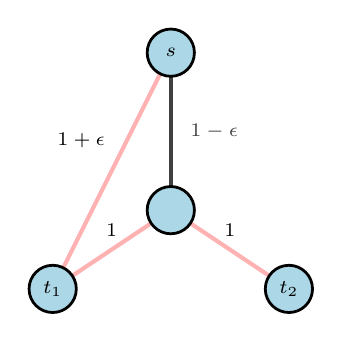
\begin{tikzpicture}
		\Vertex[label=$t_1$]{t1}
		\Vertex[label=$t_2$,x=3]{t2}
		\Vertex[x=1.5,y=1]{middle}
		\Vertex[x=1.5,y=3,label=$s$]{s}
		\Edge[label=$1$,fontcolor=black,color=red!30,position={above=1mm}](t1)(middle)
		\Edge[label=$1$,fontcolor=black,color=red!30,position={above=1mm}](t2)(middle)
		\Edge[label=$1-\epsilon$,position={right = 2mm}](s)(middle)
		\Edge[label=$1+\epsilon$,fontcolor=black,color=red!30,position={above left=2mm}](t1)(s)
	\end{tikzpicture}
	\hspace{10pt}
	 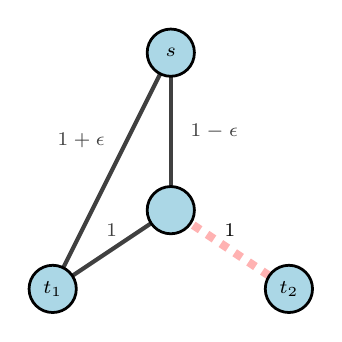
\begin{tikzpicture}
		\Vertex[label=$t_1$]{t1}
		\Vertex[label=$t_2$,x=3]{t2}
		\Vertex[x=1.5,y=1]{middle}
		\Vertex[x=1.5,y=3,label=$s$]{s}
		\Edge[label=$1$,position={above=1mm}](t1)(middle)
		\Edge[label=$1$,style={dashed},fontcolor=black,lw=3pt,color=red!30,position={above=1mm}](t2)(middle)
		\Edge[label=$1-\epsilon$,position={right = 2mm}](s)(middle)
		\Edge[label=$1+\epsilon$,position={above left=2mm}](t1)(s)
	\end{tikzpicture}
	\hspace{10pt}
	 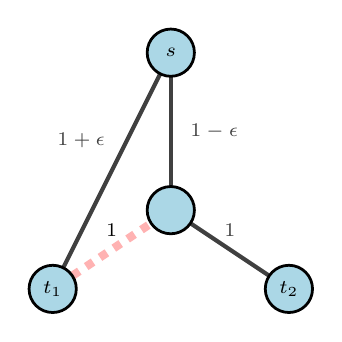
\begin{tikzpicture}
		\Vertex[label=$t_1$]{t1}
		\Vertex[label=$t_2$,x=3]{t2}
		\Vertex[x=1.5,y=1]{middle}
		\Vertex[x=1.5,y=3,label=$s$]{s}
		\Edge[label=$1$,style={dashed},fontcolor=black,lw=3pt,color=red!30,position={above=1mm}](t1)(middle)
		\Edge[label=$1$,position={above=1mm}](t2)(middle)
		\Edge[label=$1-\epsilon$,position={right = 2mm}](s)(middle)
		\Edge[label=$1+\epsilon$,position={above left=2mm}](t1)(s)
	\end{tikzpicture}
	\end{center}

	% $e$ is not a cut.\\
	% $c(A_2) = 2-\epsilon,\quad p_2(T^*) =1$\\
	% $c(e) = 1,\quad \sum_{j}p_j(e) = 0 $\\
	% set $p_2(e) = 1 - \epsilon$ \\
	In the end of the game, $e$ is not fully paid thus player 2 will deviate.
	
	\subsection{Approximate Nash Equilibrium in Connection Game}
		\begin{definition}[Approximate Equilibrium]
			A \((1+\epsilon)\)-approximate Nash Equilibrium is a payment function \(p\) such that player \(i\) would not deviate their payment by a factor of \(1+\epsilon\).
		\end{definition}
		Let $ p_i^{'}(T)$ be player's final payment,$ p_i^{'}(e) \leq (1+\epsilon)p_i(e)$
	
	
		\begin{theorem}
			Given a single source game and \(\alpha\) approximation of minimum-cost Steiner tree \(T\), \(\forall \epsilon > 0\), there is a polynomial algorithm which return a \((1+\epsilon)\)-approximation \textit{Nash equilibrium} on Steiner Tree \(T^{'}\), where $c(T^{'}) \leq c(T)$.
		\end{theorem}
	
	
	{$\gamma$ Reduction}
		Instead of trying to fully pay every edge: 
		\begin{itemize}
			\item We try to pay $T$ with $c(e) = c(e) - \gamma, \quad \gamma = \frac{\epsilon c(T)}{(1+\epsilon)n\alpha}$
			\item If all players agree to pay for $T$ with $\gamma$ reduction, we can increase their payment on every edge in $T$ by $\gamma \cdot \frac{p_i(T)}{P(T)}$
			\item $T$ will be full paid, and it is a $(1+\epsilon)$ Nash Equilibrium
			\item Forms a cheaper tree whenever a Nash equilibrium cannot be found even with $\gamma$ reduction.
		\end{itemize}
	
	
	If all players ends of buying  $T$ with $\gamma$ reduction, $p_i^{'}(e) \gets p_i(e) + \gamma\frac{p_i(T)}{P(T)}$.\\
	Suppose there are $m$ edges in $T$,
	\[p_i^{'}(T) - p_i(T) \leq \epsilon p_i(T)\]
	\[p_i^{'}(T) - p_i(T) =  \gamma\frac{p_i(T)}{P(T)}m =  \gamma\frac{p_i(T)}{c(T)-m\gamma}m \leq \epsilon p_i(T)\]
	\[ \frac{m\gamma}{c(T)-m\gamma} \leq \epsilon \Rightarrow \gamma \leq \frac{\epsilon c(T)}{(1+\epsilon)m}\]
	Since we also need to bound the value after reconstruction, we define $\gamma = \frac{\epsilon c(T)}{(1+\epsilon)n\alpha},\quad n = |V|$
	
	
		\begin{algorithm}[H]
			\begin{algorithmic}[2]
				\STATE $c^{'}(e) \gets  c(e) -\gamma \quad \forall e \in T$
				\STATE Run Algorithm 1 to attempt to pay for on $T$ under modified cost
				\WHILE{\( e \in T \) }
				\IF{\(e\) is not fully paid}
				\STATE  Adjust \( T\) by replacing \(T_e\) with  \(\bigcup_{i\in T_e} A_i\) to get \(T^{'}\)
				\STATE BREAK
				% Run Algorithm 1 to pay for $T^{'}$ under modified cost
				\ENDIF
				\ENDWHILE
				\STATE Modify($T^{'}$)
			   
			\end{algorithmic}
			\caption{Modify $T$ }
			\end{algorithm}
	
			$P(T^{'}) \gets \sum_i p_i(T^{'})$\\
			$p_i^{'}(e) \gets p_i(e) + \gamma\frac{p_i(T^{'})}{P(T^{'})}\quad \text{ for all players and every } e \in T^{'}$
	
	
	{$T^{'}$ Is Fully Paid under $P^{'}$ and Algorithm 2 Runs in Polynomial Time}
		$T^{'}$ is fully paid as $\sum_i p_i^{'}(e) = \sum_i p_i(e) + \gamma$\\
		
		Whenever \( e \in T \) is not fully paid, we form a new tree $T^{'}$, and $c(T^{'}) \leq c(T) - \gamma $.\\
		Therefore, we need to reconstruct our Steiner tree most  $\frac{c(T)}{\gamma} = \frac{(1+\epsilon)n\alpha }{\epsilon}$ times.
	
	
	
	{$P^{'}(T^{'})$ Is A $(1+\epsilon)$ Nash Equilibrium}
		\[p_i^{'}(e) = p_i(e) + \gamma\frac{p_i(T^{'})}{P(T^{'})}\]
		
		Suppose $T^{'}$ has $m^{'}$ edges:
		\[p_i^{'}(T^{'}) = p_i(T^{'}) + \gamma\frac{p_i(T^{'})}{P(T^{'})}m^{'} = p_i(T^{'}) + \gamma\frac{p_i(T^{'})}{c(T^{'}) - m^{'}\gamma}\]
		
	
	
	{$P^{'}(T^{'})$ Is A $(1+\epsilon)$ Nash Equilibrium}
		\begin{align*}
		p_i^{'}(T^{'}) - p_i(T^{'}) &=  \gamma\frac{p_i(T^{'})}{c(T^{'}) - m^{'}\gamma}m^{'}\\  &= \frac{\epsilon c(T) p_i(T^{'}) m^{'} }{(1+\epsilon)n\alpha(c(T^{'}) - m^{'}\gamma)}  \\ &=  \frac{\epsilon c(T) p_i(T^{'})}{(1+\epsilon)\alpha n(\frac{c(T^{'})}{m^{'}} - \gamma)} \\ &=  \frac{\epsilon c(T) p_i(T^{'})}{(1+\epsilon)\alpha (\frac{n}{m^{'}} - \frac{n\gamma}{c(T^{'})})c(T^{'})}   
		\end{align*}
	
	
	{$P^{'}(T^{'})$ Is A $(1+\epsilon)$ Nash Equilibrium}
		\[\frac{n\gamma}{c(T^{'})} = \frac{\epsilon c(T) n}{(1+\epsilon)n\alpha c(T^{'})} = \frac{\epsilon c(T) }{(1+\epsilon)\alpha c(T^{'})}\]
		\[c(T) = \alpha c(T^*)\]
		\[\frac{n\gamma}{c(T^{'})} = \frac{\epsilon c(T^*)}{(1+\epsilon)c(T^{'})} < \epsilon\]
		\[p_i^{'}(T^{'}) - p_i(T^{'}) \leq \frac{\epsilon c(T) p_i(T^{'}) }{(1+\epsilon)\alpha (1-\epsilon) c(T^{'}) } = \frac{\epsilon  p_i(T^{'}) }{(1+\epsilon) (1-\epsilon) } \leq \epsilon p_i(T^{'})\]
	
	
	
		
\section{Lower Bound of Approximate Nash Equilibrium}
	
\subsection{General Game}
In the general case, players can have different numbers of terminals and do not necessarily share the same source.

\begin{lemma}
	The price of stability in general cases can be bad as $\Theta(N)$.
\end{lemma}
\begin{center}
	
	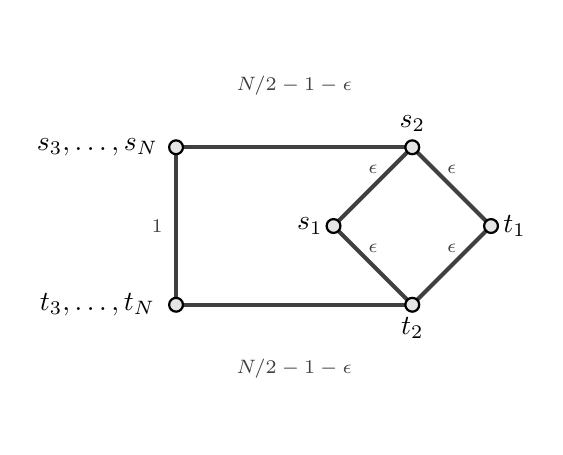
\begin{tikzpicture}
		\coordinate (s) at (0,0);
		\coordinate (t) at (0,-2);
		\coordinate (s1) at (2,-1);
		\coordinate (t1) at (4,-1);
		\coordinate (s2) at (3,0);
		\coordinate (t2) at (3,-2);
		\node[draw,circle,fill=gray!20,thick,inner sep=1pt,minimum size=5pt] (CircleNode) at (s)  {};
		\node[draw,circle,fill=gray!20,thick,inner sep=1pt,minimum size=5pt] (CircleNode) at (s1)  {};
		\node[draw,circle,fill=gray!20,thick,inner sep=1pt,minimum size=5pt] (CircleNode) at (s2)  {};
		\node[draw,circle,fill=gray!20,thick,inner sep=1pt,minimum size=5pt] (CircleNode) at (t)  {};
		\node[draw,circle,fill=gray!20,thick,inner sep=1pt,minimum size=5pt] (CircleNode) at (t1)  {};
		\node[draw,circle,fill=gray!20,thick,inner sep=1pt,minimum size=5pt] (CircleNode) at (t2)  {};
		\Edge[label=$1$,position={left=1mm}](s)(t)
		\Edge[label=$N/2-1-\epsilon$,position={above=0.1pt}](s)(s2)
		\Edge[label=$\epsilon$,position={above=1mm}](s1)(s2)
		\Edge[label=$\epsilon$,position={above=1mm}](s2)(t1)
		\Edge[label=$\epsilon$,position={above=1mm}](t1)(t2)
		\Edge[label=$\epsilon$,position={above=1mm}](t2)(s1)
		\Edge[label=$N/2-1-\epsilon$,position={below=1pt}](t)(t2)
		\node at  ([shift={(-1,0)}]s) {$s_3,\dots,s_N$};
		\node at  ([shift={(-1,0)}]t) {$t_3,\dots,t_N$};
		\node at ([shift={(-0.3,0)}]s1) {$s_1$};
		\node at ([shift={(0.3,0)}]t1) {$t_1$};
		\node at ([shift={(0,0.3)}]s2) {$s_2$};
		\node at ([shift={(0,-0.3)}]t2) {$t_2$};
	\end{tikzpicture}
\end{center}
	$OPT = 1+3\epsilon$\\
	Any equilibrium ends up paying $N-2$.
	
	\subsection{Lower Bounds on Nash Equilibrium in General Case}
		Since the price of stability can be as bad as $\Theta(N)$ and pure Nash equilibrium may not exist at all, we cannot hope to be able to provide cheap Nash equilibrium for multi-source games.\\
		Therefore, we instead hope that we can get a cheap $(1+\epsilon)$ approximate equilibrium.\\
		\begin{theorem}
			There exists such a graph that any equilibrium that purchases the optimal Steiner forest is at least a $(3/2-\epsilon)$ approximate equilibrium for any $\epsilon > 0$.
		\end{theorem}
	
	
	{Graph Construction }
	
		\begin{itemize}
			\item Start with a cycle with $2N$ vertices from $v_1 \text{ to } v_{2N}$ clockwise. 
			\item For $v_i$, add an edge from vertex $i$ to vertex $(i+N-1)mod (2N)$ and an edge from vertex $i$ to $(i+N+1)mod (2N)$.
			\item All edges have cost 1. 
			\item Add $N$ players and each of them have a source $s_i$ and a terminal $t_i$. 
			\item Let vertices from $v_1$ to $v_N$ be the $s$ for each player and vertices $v_{N+1}$ to $v_{2N}$ be the terminals.
		\end{itemize}
		$OPT = 2N-1$ with all the edges in the outer cycle with edge from $s_1$ to $t_N$. 
	
	
	{Proof}
	   
		\begin{lemma}
			For any equilibrium than is better than 3/2, player 1 and player N won't pay more than 3. 
		\end{lemma}
		\begin{itemize}
			\item Suppose player 1 pays $x$ to $s_1 \rightarrow t_1$, $y$ to $t_1 \rightarrow t_N$. 
			\item Player 1 has the choice to pay for only $x$ or $1+y$. 
		\end{itemize}
		
		\[\frac{x+y}{x} \leq \frac{3}{2}\quad\frac{x+y}{y+1} \leq \frac{3}{2}\]
		 \[x+y\leq 3\]    
	
	
	{Proof}
		\begin{lemma}
			Given there at least exists a player $i$ needs to pay at least $\frac{2N-7}{N-2}$, we find that player $i$ will at least have the incentive $\frac{6N-21}{4N-11}$ to deviate.
		\end{lemma}
		\begin{itemize}
			\item Suppose player $i$ pays $x$ to $s_i \rightarrow t_i$, $y$ to $s_{i-1} \rightarrow s_i$, $z$ to $t_i \rightarrow t_{i+1}$. 
			\item Player 1 has the choice to pay for only $x$, $1+y$,or $1+z$. 
		\end{itemize}
		
		\textbf{ Player $i$ has $max\{\frac{x+y+z}{x},\frac{x+y+z}{1+y},\frac{x+y+z}{1+z}\}$ incentive to deviate. }
	
	{Proof}
		$max\{\frac{x+y+z}{x},\frac{x+y+z}{1+y},\frac{x+y+z}{1+z}\}$ is minimized when $x = 1+y =1+z$. 
		\[x+y+z \geq \frac{2N-7}{N-2}\]
		\[x \geq \frac{4N-11}{3N-6}\]
		\[\frac{x+y+z}{x} \geq \frac{3x-2}{x} = 3-\frac{2}{x} \geq \frac{6N-21}{4N-11} \]
	
	
	\subsection{Bicriteria Approximation}
	\begin{center}
			\begin{tabular} { 
				| m{5cm} | m{3cm}| m{3cm} | }
			   \hline
				& Single Source & Multi-Source\\
			   \hline
			   Exists Nash  & (1,1)  &  (3,1)\\
			  \hline
			  Can find Nash in poly-time & $(1+\epsilon,1.55)$ & $(4.65+\epsilon,2)$\\
			  \hline
			  Lower Bounds on Existence & (1,1) & (1.5,1)\\
			  \hline
			  \end{tabular}
	\end{center}

		  
		The closest approximation ratio has been obtained so far is 1.55 by k-restricted Steiner Tree.\\
		A better approximation ratio, 1.39, was archived 2 years after this paper by modeling Steiner tree into linear programming relaxtion and itertative randomized rounding.
	
	

It has been proven that it is NP-hard to approximate Steiner tree problem within ratio \(96/95\). However, it is possible to obtain an approximate minimum-cost Steiner tree by modeling this problem into linear programming and randomized rounding. The closest approximation ratio has been obtained so far is 1.55.

\begin{thebibliography}{10}
	\setlength{\itemsep}{0pt plus .3pt}
	\setlength{\parsep}{0pt plus .3pt}
	\setlength{\parskip}{0pt plus .3pt}
\bibitem{texbook}
Vazirani Vijay V. {\em Approximation Algorithms.\/} Chapters 3.1 and 22, Springer, 2003.
\end{thebibliography}

\end{document}



